\documentclass[journal,12pt,twocolumn]{IEEEtran}
%
\usepackage{setspace}
\usepackage{gensymb}
\usepackage{xcolor}
\usepackage{caption}
\usepackage[hyphens,spaces,obeyspaces]{url}
%\usepackage{subcaption}
%\doublespacing
\singlespacing

%\usepackage{graphicx}
%\usepackage{amssymb}
%\usepackage{relsize}
\usepackage[cmex10]{amsmath}
\usepackage{mathtools}
%\usepackage{amsthm}
%\interdisplaylinepenalty=2500
%\savesymbol{iint}
%\usepackage{txfonts}
%\restoresymbol{TXF}{iint}
%\usepackage{wasysym}
\usepackage{amsthm}
\usepackage{mathrsfs}
\usepackage{txfonts}
\usepackage{stfloats}
\usepackage{cite}
\usepackage{cases}
\usepackage{subfig}
%\usepackage{xtab}
\usepackage{longtable}
\usepackage{multirow}
%\usepackage{algorithm}
%\usepackage{algpseudocode}
\usepackage{enumerate}
\usepackage{mathtools}
%\usepackage{eenrc}
\usepackage{iithtlc}
%\usepackage[framemethod=tikz]{mdframed}
\usepackage[breaklinks]{hyperref}
%\usepackage{breakcites}
\usepackage{listings}
    \usepackage[latin1]{inputenc}                                 %%
    \usepackage{color}                                            %%
    \usepackage{array}                                            %%
    \usepackage{longtable}                                        %%
    \usepackage{calc}                                             %%
    \usepackage{multirow}                                         %%
    \usepackage{hhline}                                           %%
    \usepackage{ifthen}                                           %%
  %optionally (for landscape tables embedded in another document): %%
    \usepackage{lscape}     

\usepackage{tikz}
\usepackage{circuitikz}
\usepackage{karnaugh-map}
\usepackage{pgf}
\usepackage[hyphenbreaks]{breakurl}

%\usepackage{url}
%\def\UrlBreaks{\do\/\do-}





%\usepackage{stmaryrd}


%\usepackage{wasysym}
%\newcounter{MYtempeqncnt}
\DeclareMathOperator*{\Res}{Res}
%\renewcommand{\baselinestretch}{2}
\renewcommand\thesection{\arabic{section}}
\renewcommand\thesubsection{\thesection.\arabic{subsection}}
\renewcommand\thesubsubsection{\thesubsection.\arabic{subsubsection}}

\renewcommand\thesectiondis{\arabic{section}}
\renewcommand\thesubsectiondis{\thesectiondis.\arabic{subsection}}
\renewcommand\thesubsubsectiondis{\thesubsectiondis.\arabic{subsubsection}}

% correct bad hyphenation here
\hyphenation{op-tical net-works semi-conduc-tor}

%\lstset{
%language=C,
%frame=single, 
%breaklines=true
%}

%\lstset{
	%%basicstyle=\small\ttfamily\bfseries,
	%%numberstyle=\small\ttfamily,
	%language=Octave,
	%backgroundcolor=\color{white},
	%%frame=single,
	%%keywordstyle=\bfseries,
	%%breaklines=true,
	%%showstringspaces=false,
	%%xleftmargin=-10mm,
	%%aboveskip=-1mm,
	%%belowskip=0mm
%}

%\surroundwithmdframed[width=\columnwidth]{lstlisting}
\def\inputGnumericTable{}                                 %%
\lstset{
%language=C,
frame=single, 
breaklines=true,
columns=fullflexible
}
 

\begin{document}
%

\theoremstyle{definition}
\newtheorem{theorem}{Theorem}[section]
\newtheorem{problem}{Problem}
\newtheorem{proposition}{Proposition}[section]
\newtheorem{lemma}{Lemma}[section]
\newtheorem{corollary}[theorem]{Corollary}
\newtheorem{example}{Example}[section]
\newtheorem{definition}{Definition}[section]
%\newtheorem{algorithm}{Algorithm}[section]
%\newtheorem{cor}{Corollary}
\newcommand{\BEQA}{\begin{eqnarray}}
\newcommand{\EEQA}{\end{eqnarray}}
\newcommand{\define}{\stackrel{\triangle}{=}}

\bibliographystyle{IEEEtran}
%\bibliographystyle{ieeetr}

\providecommand{\nCr}[2]{\,^{#1}C_{#2}} % nCr
\providecommand{\nPr}[2]{\,^{#1}P_{#2}} % nPr
\providecommand{\mbf}{\mathbf}
\providecommand{\pr}[1]{\ensuremath{\Pr\left(#1\right)}}
\providecommand{\qfunc}[1]{\ensuremath{Q\left(#1\right)}}
\providecommand{\sbrak}[1]{\ensuremath{{}\left[#1\right]}}
\providecommand{\lsbrak}[1]{\ensuremath{{}\left[#1\right.}}
\providecommand{\rsbrak}[1]{\ensuremath{{}\left.#1\right]}}
\providecommand{\brak}[1]{\ensuremath{\left(#1\right)}}
\providecommand{\lbrak}[1]{\ensuremath{\left(#1\right.}}
\providecommand{\rbrak}[1]{\ensuremath{\left.#1\right)}}
\providecommand{\cbrak}[1]{\ensuremath{\left\{#1\right\}}}
\providecommand{\lcbrak}[1]{\ensuremath{\left\{#1\right.}}
\providecommand{\rcbrak}[1]{\ensuremath{\left.#1\right\}}}
\theoremstyle{remark}
\newtheorem{rem}{Remark}
\newcommand{\sgn}{\mathop{\mathrm{sgn}}}
\providecommand{\abs}[1]{\left\vert#1\right\vert}
\providecommand{\res}[1]{\Res\displaylimits_{#1}} 
\providecommand{\norm}[1]{\lVert#1\rVert}
\providecommand{\mtx}[1]{\mathbf{#1}}
\providecommand{\mean}[1]{E\left[ #1 \right]}
\providecommand{\fourier}{\overset{\mathcal{F}}{ \rightleftharpoons}}
%\providecommand{\hilbert}{\overset{\mathcal{H}}{ \rightleftharpoons}}
\providecommand{\system}{\overset{\mathcal{H}}{ \longleftrightarrow}}
	%\newcommand{\solution}[2]{\textbf{Solution:}{#1}}
\newcommand{\solution}{\noindent \textbf{Solution: }}
\providecommand{\dec}[2]{\ensuremath{\overset{#1}{\underset{#2}{\gtrless}}}}
%\numberwithin{equation}{subsection}
\numberwithin{equation}{section}
%\numberwithin{problem}{subsection}
%\numberwithin{definition}{subsection}
\makeatletter
\@addtoreset{figure}{problem}
\makeatother

\let\StandardTheFigure\thefigure
%\renewcommand{\thefigure}{\theproblem.\arabic{figure}}
\renewcommand{\thefigure}{\theproblem}


%\numberwithin{figure}{subsection}

%\numberwithin{equation}{subsection}
%\numberwithin{equation}{section}
%%\numberwithin{equation}{problem}
%%\numberwithin{problem}{subsection}
\numberwithin{problem}{section}
%%\numberwithin{definition}{subsection}
%\makeatletter
%\@addtoreset{figure}{problem}
%\makeatother
\makeatletter
\@addtoreset{table}{problem}
\makeatother

\let\StandardTheFigure\thefigure
\let\StandardTheTable\thetable
%%\renewcommand{\thefigure}{\theproblem.\arabic{figure}}
%\renewcommand{\thefigure}{\theproblem}
\renewcommand{\thetable}{\theproblem}
%%\numberwithin{figure}{section}

%%\numberwithin{figure}{subsection}



\def\putbox#1#2#3{\makebox[0in][l]{\makebox[#1][l]{}\raisebox{\baselineskip}[0in][0in]{\raisebox{#2}[0in][0in]{#3}}}}
     \def\rightbox#1{\makebox[0in][r]{#1}}
     \def\centbox#1{\makebox[0in]{#1}}
     \def\topbox#1{\raisebox{-\baselineskip}[0in][0in]{#1}}
     \def\midbox#1{\raisebox{-0.5\baselineskip}[0in][0in]{#1}}

\vspace{3cm}

\title{ 
	\logo{
Fourier Transforms
		}
}



% paper title
% can use linebreaks \\ within to get better formatting as desired
%\title{Matrix Analysis through Octave}
%
%
% author names and IEEE memberships
% note positions of commas and nonbreaking spaces ( ~ ) LaTeX will not break
% a structure at a ~ so this keeps an author's name from being broken across
% two lines.
% use \thanks{} to gain access to the first footnote area
% a separate \thanks must be used for each paragraph as LaTeX2e's \thanks
% was not built to handle multiple paragraphs
%

\author{G V V Sharma$^{*}$% <-this % stops a space
\thanks{*The author is with the Department
of Electrical Engineering, Indian Institute of Technology, Hyderabad
502285 India e-mail:  gadepall@iith.ac.in. All content in this manual is released under GNU GPL.  Free and open source.}% <-this % stops a space
%\thanks{J. Doe and J. Doe are with Anonymous University.}% <-this % stops a space
%\thanks{Manuscript received April 19, 2005; revised January 11, 2007.}}
}
% note the % following the last \IEEEmembership and also \thanks - 
% these prevent an unwanted space from occurring between the last author name
% and the end of the author line. i.e., if you had this:
% 
% \author{....lastname \thanks{...} \thanks{...} }
%                     ^------------^------------^----Do not want these spaces!
%
% a space would be appended to the last name and could cause every name on that
% line to be shifted left slightly. This is one of those "LaTeX things". For
% instance, "\textbf{A} \textbf{B}" will typeset as "A B" not "AB". To get
% "AB" then you have to do: "\textbf{A}\textbf{B}"
% \thanks is no different in this regard, so shield the last } of each \thanks
% that ends a line with a % and do not let a space in before the next \thanks.
% Spaces after \IEEEmembership other than the last one are OK (and needed) as
% you are supposed to have spaces between the names. For what it is worth,
% this is a minor point as most people would not even notice if the said evil
% space somehow managed to creep in.



% The paper headers
%\markboth{Journal of \LaTeX\ Class Files,~Vol.~6, No.~1, January~2007}%
%{Shell \MakeLowercase{\textit{et al.}}: Bare Demo of IEEEtran.cls for Journals}
% The only time the second header will appear is for the odd numbered pages
% after the title page when using the twoside option.
% 
% *** Note that you probably will NOT want to include the author's ***
% *** name in the headers of peer review papers.                   ***
% You can use \ifCLASSOPTIONpeerreview for conditional compilation here if
% you desire.




% If you want to put a publisher's ID mark on the page you can do it like
% this:
%\IEEEpubid{0000--0000/00\$00.00~\copyright~2007 IEEE}
% Remember, if you use this you must call \IEEEpubidadjcol in the second
% column for its text to clear the IEEEpubid mark.



% make the title area
\maketitle

\tableofcontents

\bigskip

\renewcommand{\thefigure}{\theenumi}
\renewcommand{\thetable}{\theenumi}

\begin{abstract}
	This manual provides a quick introduction to the Fourier transform.
\end{abstract}
%\newpage
%\section{Components}
%\input{./figs/components.tex}
%
%\section{Fourier Series}
%Complete all exercises in \cite{gvv_fourier_series}.
\section{Sinusoidal Response}
\begin{enumerate}[1.]
\item Fig. \ref{fig:rc} shows an $RC$ circuit with input $x(t)$ and output $y(t)$.  Show that
\begin{equation}
\label{eq:diff}
\begin{split}
RC\frac{dy}{dt} + y(t) = x(t)
\end{split}
\end{equation}
\begin{figure}[!h]
\centering
\resizebox {\columnwidth} {!} {
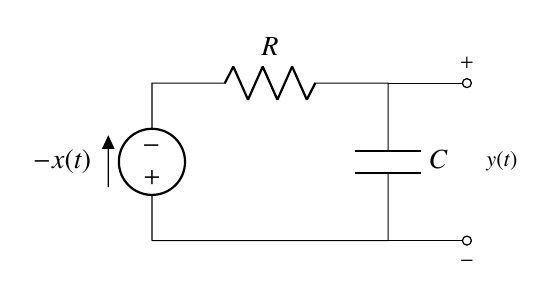
\begin{tikzpicture}
%--------start graphics code --------
%\draw[step=0.5,very thin,black!20] (-1,-0.5) grid (6,2.5);
\path (0,0) coordinate (ref_gnd);
\draw

  (ref_gnd) to[american voltage source=$-x(t)$] ++(0,2)
            to[R=$R$] ++(3,0) 
            to[C=$C$] ++(0,-2) 
  -- (ref_gnd);
\draw (3,2)   to [short, -o]   (4,2) node[ocirc,label={[font=\footnotesize]above:$+$}] {};
\draw (3,0)   to [short, -o]   (4,0) node[ocirc,label={[font=\footnotesize]below:$-$}] {};
\draw (4,1)  node[label={[font=\footnotesize]right:$y(t)$}] {};
%--------end graphics code ----------
\end{tikzpicture}

}
\caption{RC Circuit} 
\label{fig:rc}
\end{figure}
\item Let $x(t) = \cos 2\pi f_0 t$. Show that
\begin{equation}
y(t) = \frac{1}{\sqrt{1+\brak{2\pi f_0 RC}^2}}\cos\sbrak{2\pi f_0 \brak{t - \tan^{-1}RC}  }
\end{equation}
by solving the differential equation in \eqref{eq:diff} using the integrating factor.
\begin{equation}
\begin{split}
%
\end{split}
\end{equation}
\end{enumerate}

\section{Fourier Transform}
The Fourier transform of a signal $g(t)$ is defined as
\begin{equation}
\label{eq:fourier}
G(f) = \int_{-\infty}^{\infty}g(t)e^{-\j 2\pi f t}\,dt
\end{equation}
\begin{enumerate}[1.]
\item Define the Dirac delta function as
\begin{equation}
\begin{split}
\int_{\infty}^{\infty} \delta(t)\,dt &= 1
\\
\delta(t) &= 0, \quad t \neq 0.
\end{split}
\end{equation}
and show that
\begin{equation}
\delta (t) \fourier 1
\end{equation}
\item Show that 
\begin{equation}
\delta (t-t_0) \fourier e^{-\j2\pi f t_0}
\end{equation}
\item  Show that 
\begin{equation}
\label{eq:duality}
\begin{split}
g(t) & \fourier G(f)
\\
\implies G(t) & \fourier g(-f)
\end{split}
\end{equation}
assuming
\begin{equation}
\label{eq:inv_fourier}
g(t) = \int_{-\infty}^{\infty}G(f)e^{\j 2\pi f t}\,df.
\end{equation}
\eqref{eq:inv_fourier} is known as the inverse Fourier transform.
\item Show that
\begin{equation}
\cos2\pi f_0 t \fourier \frac{1}{2}\sbrak{\delta\brak{f-f_0}+\delta \brak{f+f_0}}
\end{equation}
\item Show that
\begin{equation}
\frac{dy}{dt} \fourier \j 2 \pi f Y(f)
\end{equation}
\item Define
\begin{equation}
u(t) =
\begin{cases}
0 & t < 0
\\
1 & t > 0
\end{cases}
\end{equation}
Show that
\begin{equation}
e^{-at}u(t) \fourier \frac{1}{a+\j 2\pi f}
\end{equation}
\item If $x(t) = \delta(t)$ in \eqref{eq:diff}, find $y(t)$ using Fourier transforms. This is known as the {\em impulse response} and is denoted by $h(t)$.
\item Solve \eqref{eq:diff} for $x(t) = \cos 2\pi f_0 t$ using Fourier transforms.
\item Verify that
\begin{equation}
y(t) = h(t)*x(t) = \int_{\infty}^{\infty}h(\tau)x\brak{t-\tau}\, d\tau
\end{equation}
This is known as the {\em convolution integral}.
\item Show that
\begin{equation}
x(t)*h(t) \fourier X(f)H(f)
\end{equation}
\item In  \eqref{eq:diff}, show that
\begin{equation}
H(f) = \frac{1}{1+\j 2\pi f RC}
\end{equation}
\item Show that 
\begin{equation}
y(t) = \abs{H(f_0)}\cos\sbrak{2\pi f_0 t + \angle H(f_0)}
\end{equation}
\end{enumerate}
\section{Filtering}
\begin{enumerate}[1.]
\item  Plot $\abs{H(f)}$ for different values of $RC$.
The following code plots Fig. \ref{fig:lpf}.
\lstinputlisting{./codes/lpf.py}
\begin{figure}[!h]
\centering
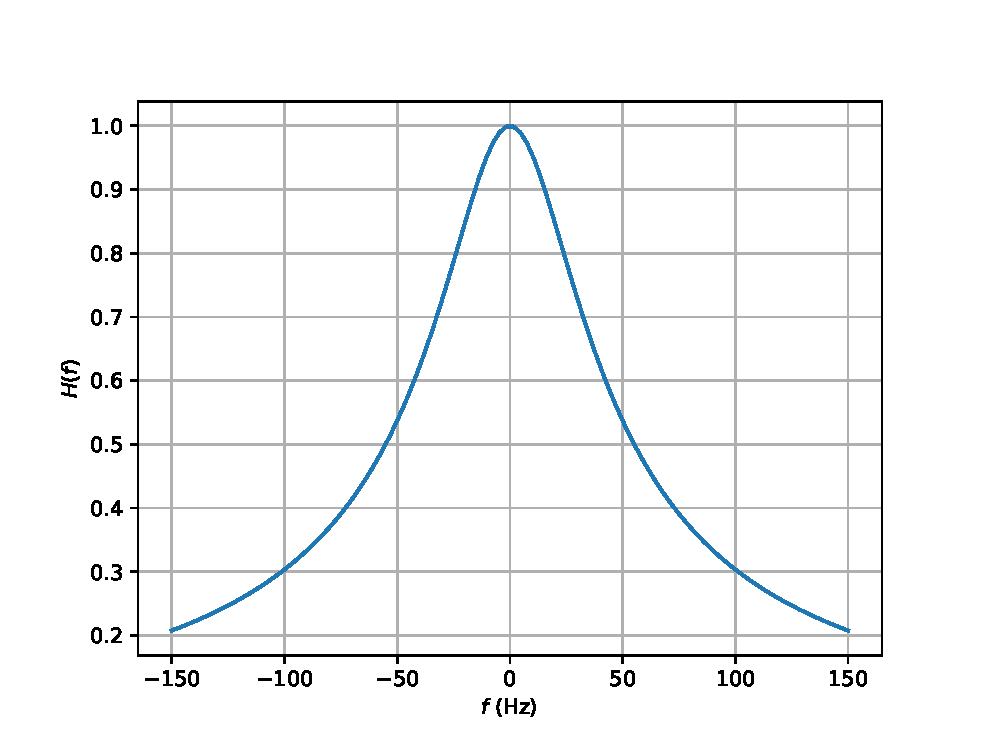
\includegraphics[width=\columnwidth]{./figs/lpf.eps}
\caption{Low Pass Filter} 
\label{fig:lpf}
\end{figure}
\item Sketch the output when $x(t) = \cos 100\pi t + \cos 300 \pi t, R = 500 \Omega$ and $C = 10 
\mu$F for $t \in \brak{-50 ms, 50 ms}$. Comment.
\item Sketch the output when $x(t) = \cos 100\pi t + \cos 2 \pi k t, R = 500 \Omega$ and $C = 10 
\mu$F for different values of $k$.  Find the value of $k$ for which the output of  $H(f)$ is  
almost $\cos 100 \pi t$.
%\begin{lstlisting}
%\input{./codes/lpf.py}
%\end{lstlisting}
\end{enumerate}

%\bibliography{IEEEabrv,gvv_fourier_prelims}
\end{document}

